\chapter{Evaluation}

Evaluating the results of bandwidth limitations is more difficult than it might seem. Both, bandwidth limitation tools like \acs{TC} as well as testing tools like iPerf3 are often buggy and/or insufficiently documented. Therefore it is often unclear whether errors are measurement errors or limitation errors. Furthermore, there is no such thing as standard \acs{IP}- or even \ac{UDP}-traffic. Packets can have different sizes, can be reordered or get lost. All those factors can influence and sometimes falsify the measurement. And finally it is questionable whether the traffic that is generated by the testing tools is similar enough to normal traffic generated by an \acs{AS}, such that we can conclude anything meaningful.
\\
What is known about the environment in which the \textit{scionlab\_bw\_limiter} will be running is that we deal with \acs{UDP}-traffic over \acs{IP}v4 and at some point in the future might be dealing with \acs{IP}v6 traffic as well. Therefore, we mainly focus on testing the bandwidth limitations using \acs{UDP}-traffic over \acs{IP}v4.

\section{Test Set-up}

As a test set-up it makes sense to have a test server, which doesn't have any bandwidth limitations and a test client, where the \textit{scionlab\_bw\_limiter} will enforce the desired bandwidth limits. As a test client I decided to use my development \acs{VM}, which I also use to develop and test the \textit{scionlab\_bw\_limiter}. This \acs{VM} runs Ubuntu 18.04, which is a newer version than the one running on the \aclp{AP}, but since \acs{TC} works the same way on both versions of Ubuntu, this should not matter. The test server is a Ubuntu 18.04 server that runs in a \acs{VM} as well and is hosted on the same physical machine as the test client. Therefore traffic between the test server and the test client is not real network traffic, but since the \acs{TC} configurations are effective between the Linux kernel and the network driver, where both of which are virtualized, the \acs{TC} configurations should have the exact same effect in this setting as in the real environment.
\\
For testing the bandwidth between the test client and the test server, I chose two different approaches, one of which turned out to be quite useless, whereas the other one seemed to be reasonable.

\subsection{Naive Approach}

In the beginning it was not that easy to figure out how iPerf3 had to be configured and how the test results were to be interpreted. Therefore I decided to take a simpler approach in order to get an idea on what I should expect from the iPerf3 test results. 
\\
I decided to simply generate a file of a certain size, send it either from the server to the client or the other way around and measure the time it takes until it arrives at the other end. Unfortunately it's not that simple. The connection between the two \acsp{VM} is quite fast, even when its bandwidth is limited. However relative to the transmission time, the time to load a file from memory or even from the harddisk is quite long. Therefore the measurements were highly inaccurate.

\subsection{Using iPerf3}

Since the naive approach turned out to be to inaccurate to be of any use, I decided to set up an iPerf3 test environment. I installed iPerf3 on both the test client as well as on the test server and let the test server run iPerf3 as a server. Note that the same software is used for both the server side as well as the client side. They just run in different modes. On the client I can now connect to the test server and run highly customisable tests with the server. Normally the client is the one sending data to the server, but iPerf3 can be run in a reverse mode (using the \textit{-R} option), such that we can test both ingress as well as egress traffic without having to switch between client and server mode on our machines.

\section{iPerf3}

iPerf3 is a state of the art network performance measurement tool. It is a successor of iPerf and iPerf2. However it has been completely rewritten in order to make the code base cleaner and simpler and is therefore not backward compatible with iPerf2. iPerf3 has been developed by \ac{ESnet}, which is a high-speed computer network provider for the United States Department of Energy. iPerf3 is open-source and can be found on \href{https://github.com/esnet/iperf}{github.com}.
\\
iPerf3 can test both \ac{TCP} as well as \acs{UDP} traffic. In our case we only need to test \acs{UDP} traffic. This can be done by passing the option \textit{-u} as an argument to iPerf3. When running it we need to specify a target bandwidth (option \textit{-b}). iPerf3 then tries to achieve this bandwidth by sending traffic out at this rate. To run iPerf3 in server mode we only have to pass \textit{-s} as an argument. For running it in the client mode we have to analogously pass the \textit{-c} option followed by the server's \acs{IP}-address. Last but not least, we can optionally set the buffer length of the buffer from which is sent and to which is received by passing the option \textit{-l} followed by a size in kilo bytes as an argument. As we will see in section \ref{Test Results}, this option is of quite a significance.

\section{Test Results}\label{Test Results}

The following test results occurred under the following configuration:
\\
The server's \acs{IP}-address is in our case 192.168.17.129, the \acs{IP}-connection to the server is limited to 500Kbps and the default bandwidth is 1000Kbps. The \ac{MTU} parameter in \acs{TC} is set to the \acs{MTU} of the network interface that is used to connect to the specific \acs{IP}-address. In our case this is 1500 bytes. The burst parameter, which is the size of the bucket in the \acs{TBF} algorithm is set to 5K. The ceil rate is the same as the normal rate, which is 500Kbps to the test server and 1000Kbps to any other \acs{IP}-device that uses the same interface.
\\
\\
On the test server, we start iPerf3 using no other options than the \textit{-s} option, that makes iPerf3 run in server mode (see listing \ref{Test Server Command}). On the client side, we configure a bit more. We set the \textit{-u} option, in order to generate \acs{UDP} traffic as test traffic. The target bandwidth is set to 2Mbps (option \textit{-b}) and the only parameter that we are going to change for different tests is the buffer length (option \textit{-l}). We start at a buffer length of 1000 kilo bytes and go up to 10000 kilo bytes. And finally we set the \textit{-R} in case we want to run the test in reverse mode, meaning that we test with ingress traffic. Listings \ref{Example Egress Test Command} and \ref{Example Ingress Test Command} show what these commands look like. Note that if we set the buffer size too small, we encounter an error. This happens because the packets arrive in a different order than they arrived in. Therefore iPerf3 can't measure the bandwidth any more. This phenomenon is discussed on \href{https://github.com/esnet/iperf/issues/457}{github.com}\cite{mah2016iperfIssue} in the issues section of the iPerf source code.

\begin{lstlisting}[language=sh, caption = Test Server Command, captionpos=b, numbers=left, frame=single, breaklines=true, breakatwhitespace=true, showstringspaces=false, label=Test Server Command]
iperf3 -s
\end{lstlisting}
\newpage
\begin{lstlisting}[language=sh, caption = Example Egress Test Command, captionpos=b, numbers=left, frame=single, breaklines=true, breakatwhitespace=true, showstringspaces=false, label=Example Egress Test Command]
iperf3 -c 192.168.17.129 -u -b 2Mbit -l 1000
\end{lstlisting}

\begin{lstlisting}[language=sh, caption = Example Ingress Test Command, captionpos=b, numbers=left, frame=single, breaklines=true, breakatwhitespace=true, showstringspaces=false, label=Example Ingress Test Command]
iperf3 -c 192.168.17.129 -u -b 2Mbit -l 1000 -R
\end{lstlisting}

\subsection{Interpretation of the Test Results}

Figure \ref{Evaluation of the Bandwidth} shows the average bandwidth over ten samples for both ingress as well as egress traffic with respect to the buffer size. For the egress traffic the results look quite good. The average egress bandwidth lies slightly above the bandwidth limit. This is because we allow short bursts at a higher speed. Therefore, the limitations on egress traffic can be considered as effective and stable.
\\
However, for ingress traffic it is a bit a different story. That the ingress bandwidth is lower than the egress bandwidth is expected, because there is a slight overhead by redirecting ingress traffic from a physical interface to a virtual interface. So having a situation like we have it with a buffer length of 1000 kilo bytes would be desirable. However, we can't ignore that by increasing the buffer length, the ingress bandwidth drops quite drastically. For getting on the bottom of this issue, let us consider figure \ref{Evaluation of the Bandwidth Drops}. This figure shows the number of samples at a bandwidth of zero depending on the length of the buffer. It is visible that the bigger the buffer, the more the ingress traffic suffers from samples with zero bandwidth. This phenomenon happens with egress traffic as well, but it is much less significant. The increasing number of zero bandwidth samples shows that the decreased average bandwidth is not caused by a wrong limitation, since the samples that make it through are received at a bandwidth that is around the desired limit, but that for some samples either iPerf3 fails to do a measurement at all or something prevents the machine from receiving data for some time. To figure out whether these anomalies are the result of side effects the \textit{scionlab\_bw\_limiter} causes or are measurement errors of iPerf3, we need compare these results to results we get if we enforce bandwidth limits using a different tool.

\begin{figure}[h]
	\centering
	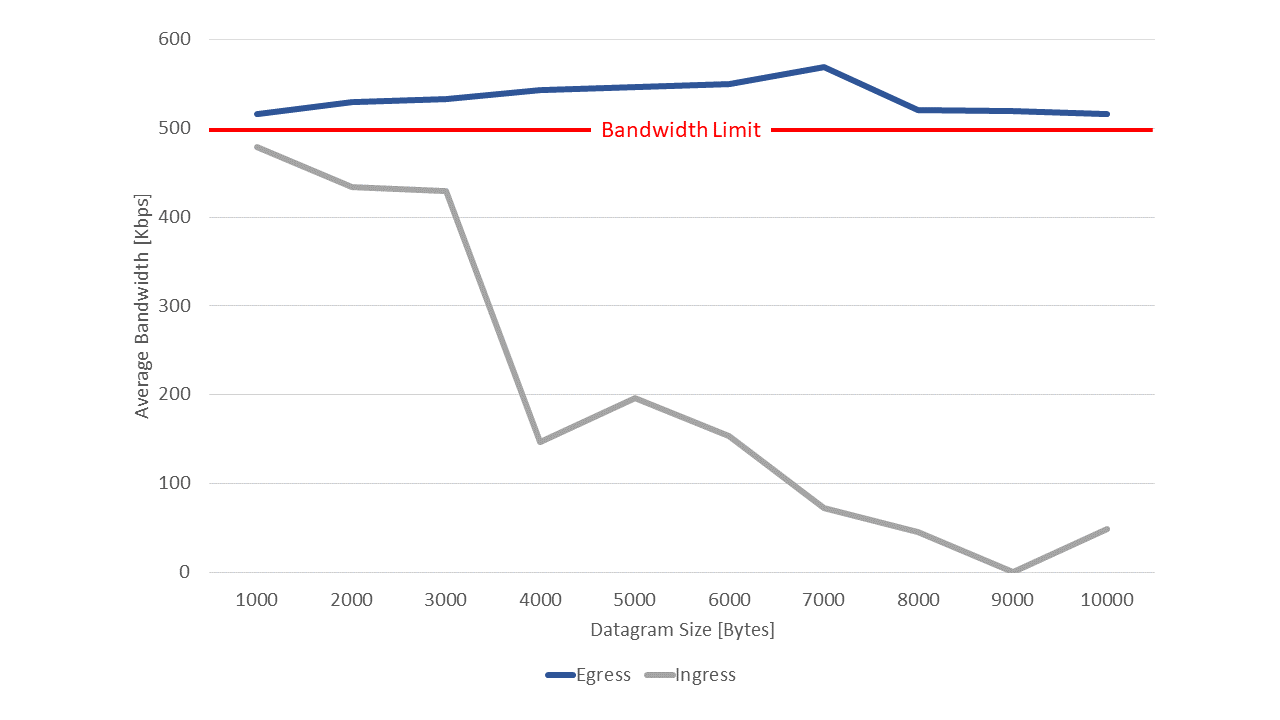
\includegraphics[width=\textwidth]{img/Evaluation-Bandwidth.png}
	\caption{Evaluation of the Bandwidth}
	\label{Evaluation of the Bandwidth}
\end{figure}

\begin{figure}[h]
	\centering
	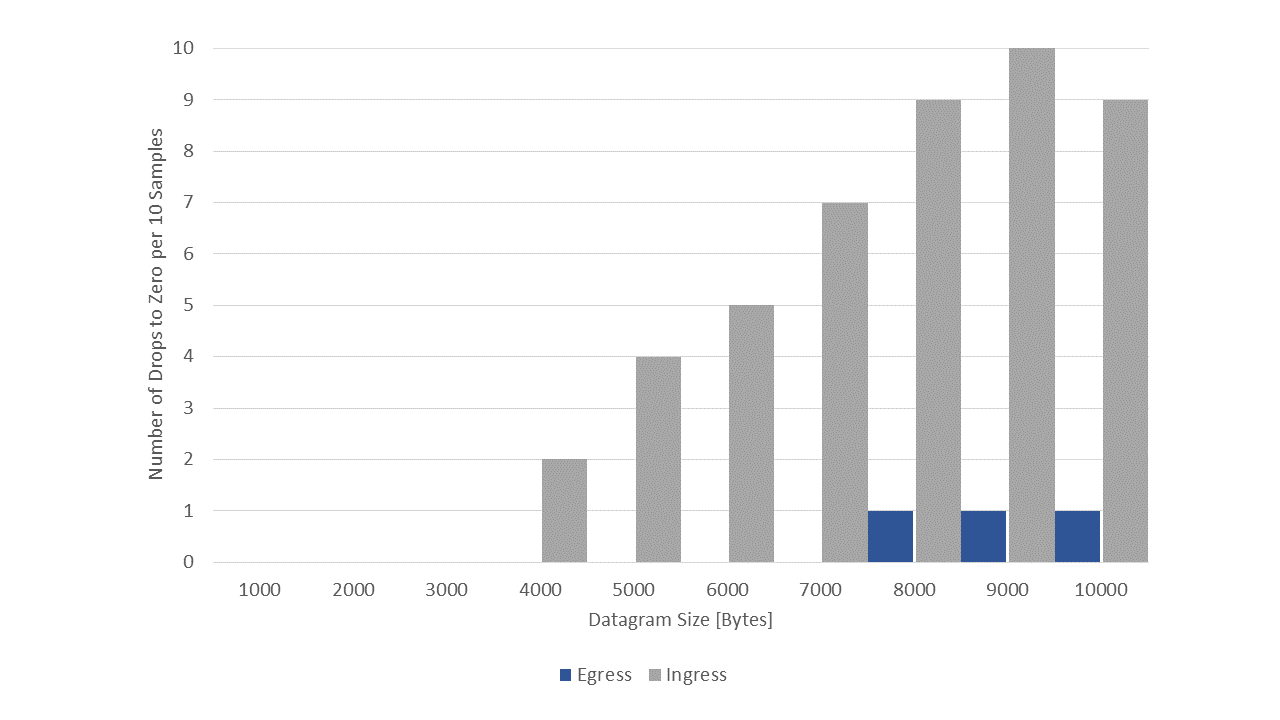
\includegraphics[width=\textwidth]{img/Evaluation-Zeros.png}
	\caption{Evaluation of Bandwidth Drops}
	\label{Evaluation of the Bandwidth Drops}
\end{figure}
%TODO maybe there is a better solution to layout that stuff...
\newpage
\textit{ }
\newpage
\subsection{Comparison with Wondershaper}

\textit{Wondershaper} is an open-source program that has been developed by some of the major contributors of the \textit{Linux advanced routing \& traffic control HOWTO}\cite
{hubert2002linux}. The code of \textit{wondershaper} can be found on \href{https://github.com/magnific0/wondershaper}{github.com}\cite{hubert2002wondershaper}. \textit{Wondershaper} only allows the user to enforce a general bandwidth limit and not individual bandwidth limits per \acs{IP}-address. On the other hand it allows us to set an ingress bandwidth that is different from the egress bandwidth. But since we don't require that we just set the same bandwidth limits in both cases on the interface that is used to connect to the test server. Listing \ref{Wondershaper command} shows the command that has been used in order to enforce a bandwidth limit of 500Kbps on interface \textit{ens33}.

\begin{lstlisting}[language=sh, caption = Wondershaper command, captionpos=b, numbers=left, frame=single, breaklines=true, breakatwhitespace=true, showstringspaces=false, label=Wondershaper command]
sudo ./wondershaper -a ens33 -u 500 -d 500
\end{lstlisting}

As we can se in Figure \ref{Evaluation of the Bandwidth (Wondershaper)} and \ref{Evaluation of the Bandwidth Drops (Wondershaper)} the same phenomenon occurs if we enforce a bandwidth limit with \textit{wondershaper} and run the exact same tests as before. It is worth noticing that even though the test results for ingress traffic look similarly bad yet quite different from the results from the \textit{scionlab\_bw\_limiter} both \textit{wondershaper} as well as the \textit{scionlab\_bw\_limiter} use the \ac{IFB} interfaces and the \textit{ingress} \acs{QDISC} and are therefore implemented almost equivalently. The egress bandwidth limits however are implemented quite differently even though the test results look almost the same. When it comes to egress traffic, \textit{wondershaper} distinguishes between different types of service, in order to achieve a better quality of service. In our case this is not necessary, since we are not dealing with average "every day traffic", but only with \acs{SCION} traffic that is wrapped into \acs{IP} packets.  

\begin{figure}[h]
	\centering
	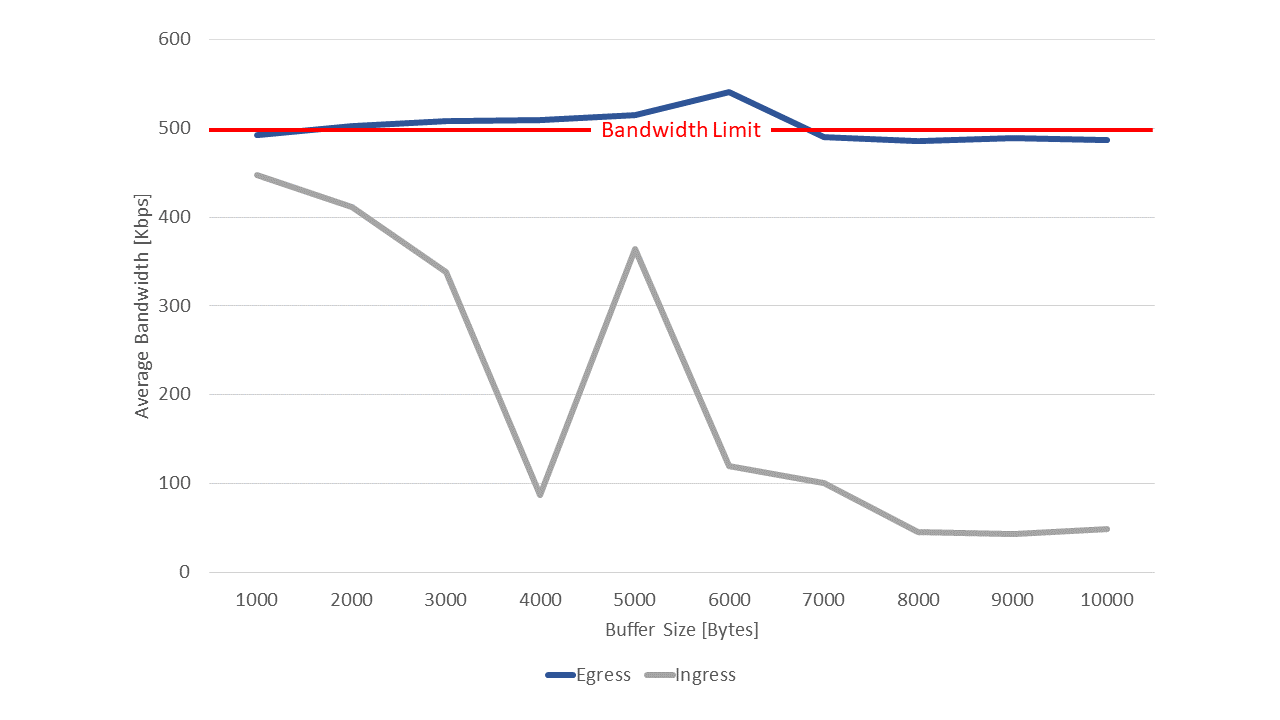
\includegraphics[width=\textwidth]{img/Evaluation-Bandwidth-Wondershaper.png}
	\caption{Evaluation of the Bandwidth (Wondershaper)}
	\label{Evaluation of the Bandwidth (Wondershaper)}
\end{figure}

\begin{figure}[h]
	\centering
	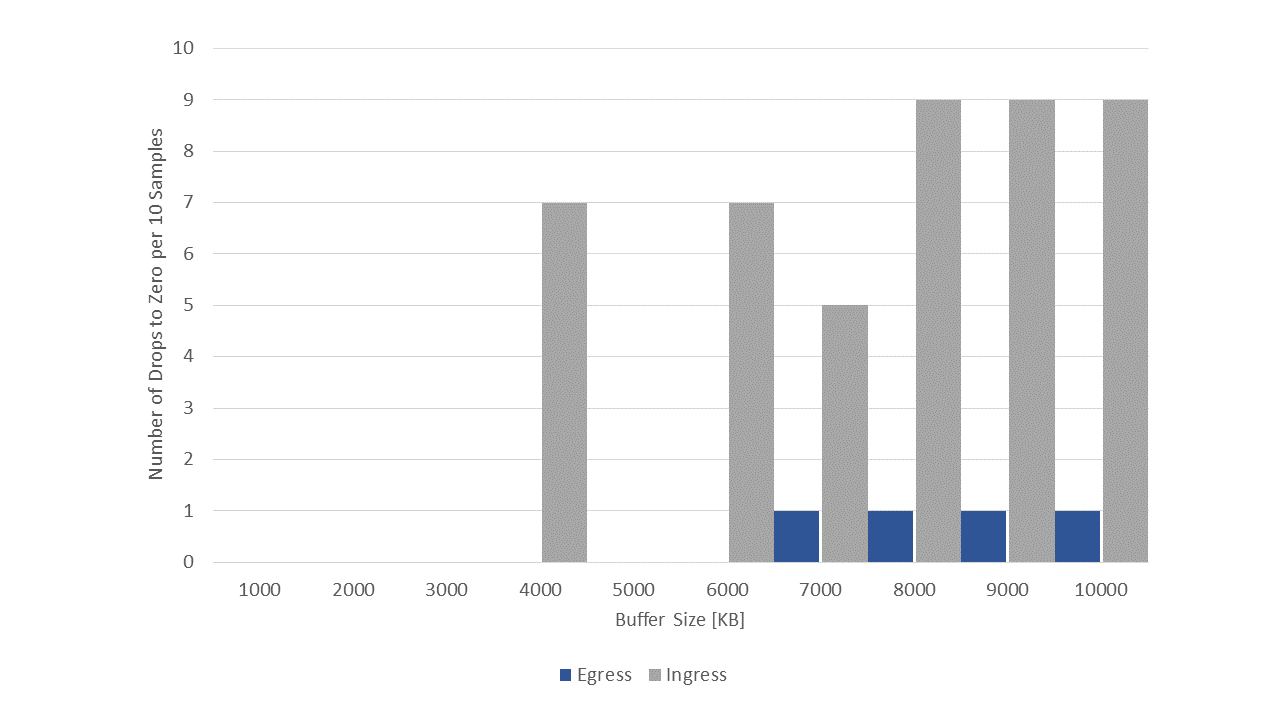
\includegraphics[width=\textwidth]{img/Evaluation-Zeros-Wondershaper.png}
	\caption{Evaluation of Bandwidth Drops (Wondershaper)}
	\label{Evaluation of the Bandwidth Drops (Wondershaper)}
\end{figure}

%Note: 
%Ingress test: iperf3 -c 192.168.17.129 -u -b 2Mbit -l 1000 -R
%Egress test: iperf3 -c 192.168.17.129 -u -b 2Mbit -l 1000
%important is the -l option that defines the buffer size (KB). otherwise ingress traffic will have one initial burst and then drop to 0

%https://github.com/esnet/iperf/issues/457